\documentclass[conference]{IEEEtran}
\IEEEoverridecommandlockouts

\usepackage{cite}
\usepackage{amsmath,amssymb,amsfonts}
\usepackage{algorithmic}
\usepackage{graphicx}
\usepackage{textcomp}
\usepackage{xcolor}
\usepackage{hyperref}
\def\BibTeX{{\rm B\kern-.05em{\sc i\kern-.025em b}\kern-.08em
    T\kern-.1667em\lower.7ex\hbox{E}\kern-.125emX}}







\pagestyle{plain}
\begin{document}
\title{
\makebox[0pt][l]{%
    \hspace*{-1.8cm}% décalage vers la gauche
    \raisebox{1.em}[0pt][0pt]{%
        
\includegraphics[width=0.20\textwidth]{logo_vnu.jpg}}%
}
\hspace{1.6cm}Self2Seg: Single-Image Self-Supervised Joint Segmentation and Denoising\\

}


\author{\IEEEauthorblockN{Reviewed by Ebwala Ebwalette Priscille}
\IEEEauthorblockA{\textit{International School, Institut Francophone International} \\
\textit{Vietnam National University} \\
Bibliography and Case Study\\
Supervisor: \textbf{Dr. Ho Tuong Vinh}\\
Cohort: SIM P27\\
Sources : \href{https://fr.overleaf.com/read/pnghmnytwfvn#447962}{Link to the overleaf source}\\
version french : articleFrancais.tex.
\\
version english : articleAnglais.tex.
}
}


\begin{document}

\maketitle

\begin{abstract}
This report was conducted as part of the academic module entitled “Bibliography and Case Study.” Its objective is to guide students in conducting an in-depth analysis of a scientific article. The selected paper, titled \textit{Self2Seg: Single-Image Self-Supervised Joint Segmentation and Denoising}, introduces an innovative method that enables simultaneous image segmentation and denoising without requiring annotated data. The authors first highlight the limitations of traditional approaches, which treat these two tasks separately and rely heavily on labeled datasets. To address these challenges, the article proposes a joint approach based on self-supervised neural networks and a shared energy function between the two tasks. This solution leverages denoising experts specific to image regions, enabling dynamic interaction between the segmentation and denoising steps. The authors then detail the model architecture, its implementation, and the experimental results obtained on noisy biomedical images. The paper concludes with potential improvements and extensions to other application domains.
\end{abstract}



\begin{IEEEkeywords}
Segmentation, denoising, self-supervision, biomedical images, deep learning, Self2Seg
\end{IEEEkeywords}


\section{Introduction}
Image segmentation and denoising are two fundamental tasks in computer vision, particularly in the biomedical domain where accurate analysis of structures is crucial. Traditionally, these tasks are handled separately using supervised models that require large volumes of annotated data. This reliance on annotations poses a significant challenge, especially in contexts where labeled data are scarce or expensive to obtain.

To overcome these limitations, self-supervised approaches have recently emerged, allowing partial or complete independence from ground truth data. Some of these methods focus on self-supervised denoising techniques such as \textit{Noise2Self}, while others explore unsupervised models for segmentation.

The article analyzed in this academic module introduces an innovative method called \textit{Self2Seg}, which jointly and self-supervisedly combines image segmentation and denoising. The proposed model relies on a shared energy function and specialized neural networks for each image region (foreground and background). This strategy not only enhances the quality of the processed images but also improves segmentation accuracy without requiring manual annotations.

This report aims to provide a structured summary of the proposed approach, analyze its implementation, discuss the experimental results, and place the solution in the broader context of related work in the field.


\section{Context, Problem Statement, and Objectives of the Paper}

This work lies at the intersection of image processing, deep learning, and unsupervised optimization. The authors explore image segmentation and denoising within a self-supervised framework through the method \textit{Self2Seg}. Segmentation aims to identify the relevant regions of an image, while denoising reduces visual perturbations such as Gaussian noise. Both tasks are particularly critical in biomedical imaging, where data quality directly impacts the reliability of analyses. However, their effectiveness often relies on manually annotated data, which can be expensive or unavailable. Moreover, conventional methods typically treat segmentation and denoising separately, missing the potential benefits of their interaction.

In response to this challenge, the authors raise a central question: \textit{How can one effectively segment and denoise an image from a single unlabeled sample?} To address this, they propose a joint self-supervised approach based on cross-optimization between the two processes.

The main objective of the paper is thus to design a robust and synergistic method that minimizes reliance on ground truth data. The results demonstrate that this approach improves both the quality of the restored images and the accuracy of segmentation, particularly in scenarios involving high levels of noise and no available annotations.


\section{State of the Art}

The authors conducted an in-depth review of the literature to identify existing approaches addressing image segmentation and denoising, particularly within a self-supervised framework. Three main research directions were explored: \textbf{variational methods, deep learning-based denoising, and combined approaches.} 

First, variational methods, such as the Chan-Vese model and its variants, have been used to segment images while reducing noise. Although effective, they often require preprocessing and are not well suited to highly noisy or unlabeled images. 

Second, techniques like \textit{Noise2Self}, \textit{Noise2Void}, and \textit{Noise2Fast} enable self-supervised denoising without the need for annotated data. However, they focus solely on visual quality and do not integrate segmentation components.

Third, some studies have attempted to combine both tasks. For instance, \textit{DenoiSeg} employs a U-Net to perform segmentation and denoising in parallel, but still relies on partial masks.

In light of these observations, the authors of \textit{Self2Seg} highlight the limitations of existing work, particularly the lack of a unified and fully self-supervised framework capable of effectively combining the two tasks without annotations. Their method seeks to overcome these shortcomings by leveraging the mutual interaction between segmentation and denoising through a joint optimization process.


\section{Proposed Solution}

In their article, the authors introduce \textit{Self2Seg}, a model in which denoising and segmentation are closely intertwined. The core idea lies in the joint optimization of a shared energy function, where each task influences and reinforces the other.

\subsection{\textbf{Region-Specific Denoising}}

Two independent neural networks are trained to process the foreground (DF) and background (DB) regions, respectively. These networks, referred to as “experts,” have their own parameters (denoted F and B) and are trained using a denoising strategy tailored to each region type. Although the model is initially designed for two regions, its extension to multiple classes is straightforward and builds upon prior work.

\begin{figure}[htbp]
    \centering
    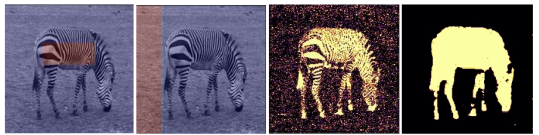
\includegraphics[width=0.4\textwidth]{debruit_region.png}
    \caption{Process illustration: input image, region detection by denoisers, and segmentation mask obtained after optimization.}
    \label{fig:debruitage_regions}
\end{figure}

\subsection{\textbf{Task Coupling}}

Segmentation and denoising are treated as interdependent processes. Their simultaneous optimization within a unified framework significantly enhances result quality. The authors identify three key aspects of this interaction:

\begin{itemize}
    \item \textbf{Influence of segmentation on denoising:} By leveraging segmentation maps, the model can more effectively target regions of interest, enabling more precise denoising without compromising important details.
    
    \item \textbf{Influence of denoising on segmentation:} By improving the visual quality of the images, denoising facilitates object and contour detection, resulting in sharper and more robust segmentations, even under noisy conditions.

    \item \textbf{Joint optimization:} Unlike sequential methods, Self2Seg relies on a shared energy function that drives both processes simultaneously. This coupling enables more coherent learning and continuous information exchange between the two modules.
\end{itemize}

\begin{figure}[htbp]
    \centering
    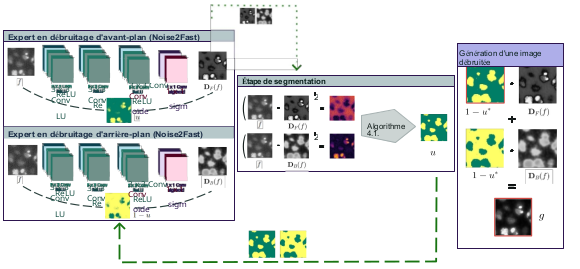
\includegraphics[width=0.4\textwidth]{couplage_deux_taches.png}
    \caption{Diagram illustrating the interaction between denoising experts for different image regions and the segmentation process within the Self2Seg model.}
    \label{fig:couplage_self2seg}
\end{figure}

Thanks to this synergy, \textit{Self2Seg} outperforms traditional approaches by fully leveraging the interaction between segmentation and denoising. This strategy makes the model more robust, more generalizable, and better suited for scenarios where annotations are not available.

\section{Implementation and Experimentation of the Article}

\subsection{\textbf{Implementation}}

The implementation of the \textit{Self2Seg} method follows a structured process composed of several key steps:

\subsubsection{\textbf{Discretization and Initialization}}\\

The procedure begins with image discretization and the definition of initial segmentation masks. These masks can be obtained either through automatic intensity thresholding or by manually selecting boxes that delimit representative regions of the foreground and background. The denoising experts, denoted as $D_F$ (for the foreground) and $D_B$ (for the background), are then trained using these initial masks to learn features specific to each type of region.

\subsubsection{\textbf{Alternating Optimization}}\\

The optimization process is carried out iteratively, alternating between updating the denoising experts and updating the segmentation mask. The ADAM optimizer is used to train the denoising networks until convergence. Once the network parameters are fixed, the energy function is minimized to adjust the segmentation mask. This optimization step is performed using the primal-dual algorithm of Chambolle-Pock.


\subsubsection{\textbf{Critère de convergence }}\\

  Les itérations se poursuivent jusqu’à ce que la diminution relative de l’énergie tombe en dessous de 15~\% par rapport à l’itération précédente, garantissant ainsi un compromis satisfaisant entre efficacité computationnelle et qualité du résultat final.
    
\subsubsection{\textbf{Convergence Criterion}}\\

The iterations continue until the relative decrease in energy falls below 15\% compared to the previous iteration, ensuring a satisfactory trade-off between computational efficiency and final result quality.

\subsection{\textbf{Experimentation}}

\subsubsection{\textbf{Data and Metrics}}\\

Experiments are conducted on the cell nuclei dataset from the \textit{Kaggle 2018 Data Science Bowl (DSB2018)} challenge. The images are deliberately degraded with Gaussian noise at increasing variance levels: 10, 30, and 50. Performance is evaluated using three indicators: the Dice coefficient for segmentation, the Structural Similarity Index (SSIM), and the Peak Signal-to-Noise Ratio (PSNR) for denoising.

\subsubsection{\textbf{Method Comparison}}\\

The \textit{Self2Seg} method is compared against several benchmark approaches, including the convex Chan-Vese model, a sequential method based on \textit{Noise2Fast}, and a deep learning-based model called \textit{DenoiSeg}. The experimental results show that \textit{Self2Seg} outperforms these competing approaches, particularly under high-noise conditions, with performance evaluated using the following metrics:

\begin{itemize}
    \item \textbf{PSNR} (Peak Signal-to-Noise Ratio): measures the quality of denoising;
    \item \textbf{SSIM} (Structural Similarity Index): evaluates the visual fidelity of the restored image;
    \item \textbf{Dice coefficient}: measures segmentation accuracy.
\end{itemize}

    
\subsubsection{\textbf{Experimental Results}}\\

The authors evaluated the performance of their \textit{Self2Seg} method under various noise conditions to assess its robustness and adaptability. The results highlight the relevance of the approach, both for mildly and heavily degraded images. Several key observations emerged from the experiments:

\begin{itemize}
    \item For low noise levels (variance = 10), a single denoising expert is used, based on the assumption of a homogeneous background. In this case, the method already achieves sharp and accurate segmentations.
    
    \item For higher noise levels (variance = 30 and 50), the authors employ two denoising experts, along with a specific filtering of the fidelity term for the background. This strategy helps avoid over-segmentation and stabilizes the generated mask.

    \item Overall, the results show that \textit{Self2Seg} outperforms baseline methods both in visual quality and quantitative performance. The approach stands out particularly in complex regions of noisy images, producing more accurate segmentations and more faithful image reconstructions.
\end{itemize}

\subsubsection{\textbf{Extensions and Limitations}}\\

The model can be generalized to multi-class segmentation tasks by incorporating multiple specialized experts. A limitation arises when one of the denoisers partially covers both target regions, which can lead to poor mask convergence. A constraint-based strategy is proposed to mitigate this issue. Additionally, the integration of techniques such as \textit{deep image prior} is suggested to enhance robustness in specific cases.

In summary, the authors present \textit{Self2Seg} as a robust approach that combines variational models and self-supervised deep learning, delivering effective results in both segmentation and denoising, even under high-noise conditions.


\section{Related Work}

In the field of self-supervision applied to segmentation and denoising, several related studies propose complementary approaches to \textit{Self2Seg}. These works share a common goal: reducing dependence on manual annotations while improving the performance of computer vision models.

\subsubsection{\textbf{BEVContrast: Self-Supervision in BEV Space for Automotive Lidar Point Clouds [2]}}\\

The authors present a contrastive learning-based method applied to LiDAR point clouds in the \textit{Bird’s Eye View} (BEV) space. This approach enables improved segmentation while minimizing annotation requirements. However, it is specifically designed for autonomous perception and is not directly applicable to microscopic images, such as those targeted by \textit{Self2Seg}.

\begin{figure}[htbp]
    \centering
    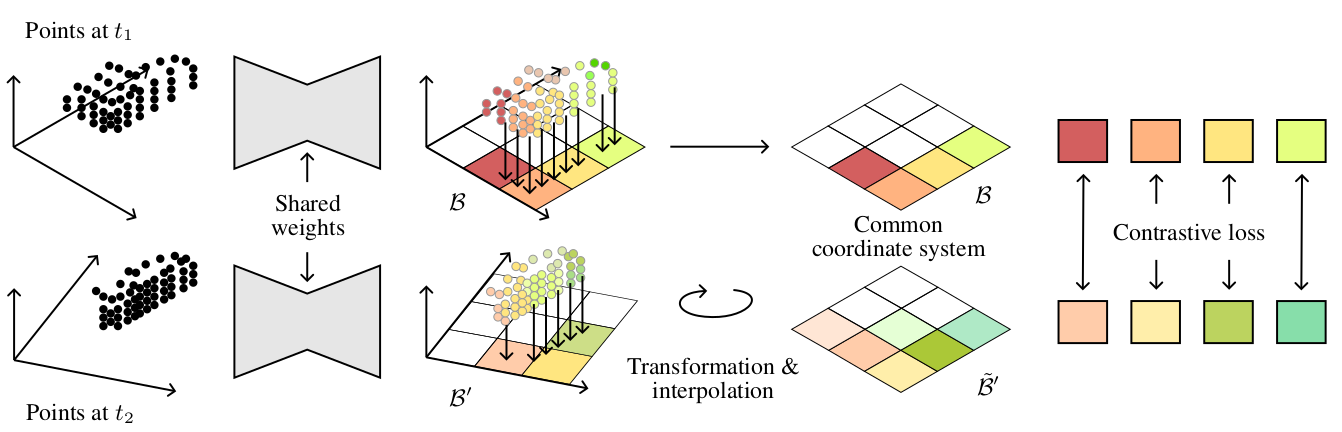
\includegraphics[width=0.4\textwidth]{article_1.png}  % Replace with your image name
    \caption{System architecture}
    \label{fig:monimage}
\end{figure}

\subsubsection{\textbf{Multi-Task Self-Supervised Learning for Image Segmentation Task [3]}}\\

This method proposes a multi-task self-supervised learning framework integrating semantic segmentation, depth prediction, and surface normal estimation. It enhances the overall robustness of the model. However, the trade-off between tasks can negatively affect segmentation accuracy, particularly when objectives are highly interdependent.

% \begin{figure}[htbp]
%     \centering
%     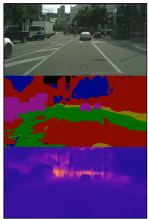
\includegraphics[width=0.1\textwidth]{article2.png}  % Replace with your image name
%     \caption{Result visualization}
%     \label{fig:monimage}
% \end{figure}

\subsubsection{\textbf{Source Identification: A Self-Supervision Task for Dense Prediction [4]}}\\

Inspired by blind source separation techniques, this approach aims to reconstruct original images from synthetic compositions. It has proven effective in the context of medical imaging, though its application to other domains remains limited.

\begin{figure}[htbp]
    \centering
    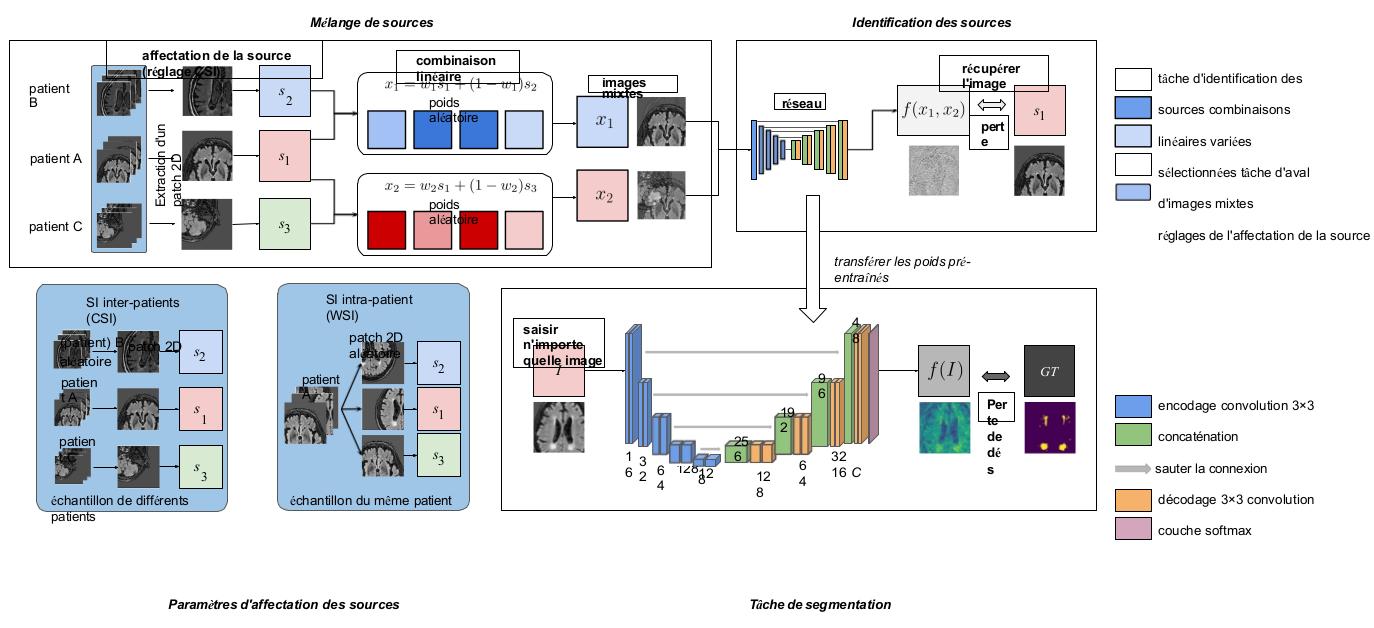
\includegraphics[width=0.4\textwidth]{article_3.png}  % Replace with your image name
    \caption{Illustration of the source identification task using three images with inter- and intra-patient strategies (CSI and WSI), and subsampling/upsampling operations applied in the UNet architecture.}
    \label{fig:monimage}
\end{figure}

These studies demonstrate that self-supervised learning can be adapted to various contexts and tasks in computer vision. However, \textit{Self2Seg} stands out due to its explicit coupling of segmentation and denoising within a fully self-supervised framework, which provides a significant advantage for applications requiring accurate segmentation without manual annotations.


\section{. Personal Critique of the Article}

The article \textit{Self2Seg} presents a valuable contribution to the field of computer vision. After a thorough analysis, several key elements emerge, highlighting both the strengths and the limitations of the proposed approach, as well as potential areas for improvement.

\subsection{\textbf{Strengths}}
\begin{itemize}
    \item \textbf{Innovative approach:} The joint integration of denoising and segmentation within a fully self-supervised framework represents a significant advancement compared to traditional methods, which are often sequential and heavily reliant on annotations.

    \item \textbf{Independence from annotated data:} The model can be trained without ground truth labels, making it particularly suitable for domains such as biomedical imaging, where annotations are rare, costly, or difficult to obtain.

    \item \textbf{Robustness to noise:} Experimental results demonstrate the effectiveness of \textit{Self2Seg} in high-noise conditions, outperforming several reference methods on heavily degraded images.
\end{itemize}


\subsection{\textbf{Limitations}}
\begin{itemize}
    \item \textbf{Sensitivity to hyperparameters:} The model's performance is highly dependent on the choice of hyperparameters, which may make its implementation challenging without appropriate or automated tuning.

    \item \textbf{Limited portability:} While effective on microscopic images, the method may require adjustments to be generalized to other types of images, particularly in industrial or natural contexts.

    \item \textbf{Incomplete comparison:} The evaluation could have been more comprehensive if the authors had compared their model to more recent and powerful segmentation architectures, such as Transformer-based models or advanced autoencoders.
\end{itemize}


\subsection{\textbf{Future Improvements}}
\begin{itemize}
    \item \textbf{Generalization to other domains:} Evaluating the model on datasets from industrial vision, satellite imagery, or natural photography would help validate its robustness beyond the biomedical domain.

    \item \textbf{Automated optimization:} Integrating techniques such as AutoML or Bayesian hyperparameter search could ease model deployment by reducing the need for manual tuning.

    \item \textbf{Hybridization with other approaches:} Combining \textit{Self2Seg} with complementary strategies, such as contrastive learning or multi-task learning, could enhance the quality of learned representations and improve overall performance.
\end{itemize}


\section{Conclusion}

The article \textit{Self2Seg} makes a significant contribution to the field of image processing by introducing a self-supervised method that simultaneously integrates denoising and segmentation. By removing the need for manual annotations, this approach represents a valuable advancement, particularly for biomedical imaging applications where labeled data are often scarce. The model stands out for its robustness to noise, adaptability, and effectiveness demonstrated across various experimental scenarios.

The analysis of this article has fostered skills in critical reading, synthesis of scientific approaches, and comparative evaluation of methods. It has also deepened the understanding of current challenges in self-supervised learning, especially in the context of noisy image segmentation. This work thus contributes to a broader reflection on innovative solutions in computer vision.



\begin{thebibliography}{00}

\bibitem{b1} N. Gruber, J. Schwab, N. Debroux, N. Papadakis, and M. Haltmeier, 
“Self2Seg: Single-Image Self-Supervised Joint Segmentation and Denoising,” 
\textit{arXiv preprint arXiv:2309.10511}, 2024.

\bibitem{b2} C. Sautier, G. Puy, A. Boulch, R. Marlet, and V. Lepetit, 
“BEVContrast: Self-Supervision in BEV Space for Automotive Lidar Point Clouds,” 
in \textit{arXiv:2310.17281v1 [cs.CV]}, 2023.

\bibitem{b3} L. Gao, C. Khamesra, U. Kumbhar, and A. Aglawe, 
“Multi-Task Self-Supervised Learning for Image Segmentation Task,” 
in \textit{arXiv:2302.02483v1 [cs.LG]}, 2023.

\bibitem{b4} S. Chen, S. Kayal, and M. de Bruijne, 
“Source Identification: A Self-Supervision Task for Dense Prediction,” 
\textit{arXiv:2307.02238v1 [cs.CV]}, 2023.

\end{thebibliography}


\end{document}
